\documentclass{book}

%------------------------------------------------------------------------------------------------------------------
%Some Packages fro adding functionality and features to notes for easier typing
\usepackage[utf8]{inputenc}
\usepackage[english]{babel}
\usepackage{mathtools}
\usepackage[document]{ragged2e}
\usepackage{geometry}
\usepackage{marginnote}
\usepackage{amsmath}
\usepackage{amsfonts}
\usepackage{amssymb}
\usepackage{tikz}

\usetikzlibrary{graphs}
\usetikzlibrary{graphs.standard}
%------------------------------------------------------------------------------------------------------------------
%------------------------------------------------------------------------------------------------------------------
% Some fancy math operator declarations which are repeated 
\DeclareMathOperator{\N}{\mathbb{N}}
\DeclareMathOperator{\Q}{\mathbb{Q}}
\DeclareMathOperator{\Z}{\mathbb{Z}}
\DeclareMathOperator{\R}{\mathbb{R}}
\DeclareMathOperator{\C}{\mathbb{C}}
\DeclareMathOperator{\im}{im}
%------------------------------------------------------------------------------------------------------------------
% Some fancy macros // May eventually move these into separate files or something and merge when building template
\renewcommand{\d}[1]{\ensuremath{\operatorname{d}\!{#1}}} % dx macro for integrals
\newcommand{\inner}[2]{\left\langle #1, #2 \right\rangle} % inner product
\newcommand{\norm}[1]{\left\lVert#1\right\rVert} % norm
\newcommand{\cpl}[1]{\overline{#1}} % complement
\renewcommand{\v}[1]{\mathbf{#1}} % vector
\newenvironment{amatrix}[1]{% augumented matrix - make sure to have # columns less than required amount
	\left(\begin{array}{@{}*{#1}{c}|c@{}}
	}{%
	\end{array}\right)
}
%----------------------------------------------------------------------------------------------------------------
%-----------------------------------------------------------------------------------------------------------------
% Define theorem environments, along with a custom proof environment
\usepackage[thref, thmmarks,amsmath]{ntheorem}
\newcommand{\itref}[1]{\textit{\thref{#1}}}

\newtheorem{lemma}{Lemma}[section]
\newtheorem{theorem}{Theorem}[section]
\newtheorem{definition}{Definition}[section]
\newtheorem{observation}{Observation}[section]
\newtheorem{corollary}{Corollary}[section]

\theoremseparator{}
\theoremindent0.0cm
\theoremstyle{nonumberplain}
\theoremheaderfont{\scshape}
\theorembodyfont{\upshape}
\theoremsymbol{$\square$}
\newtheorem{proof}{Proof}

%-----------------------------------------------------------------------------------------------------------------
\title{Math 239}
\author{Vishesh Gupta}
\begin{document}
\maketitle
\tableofcontents 
\chapter{Combinatorial Analysis}
\section{Introduction}
\section{Sums and Products}
\section{Binomial Coefficients}
\section{Bijections(One-to-One Correspondence)}
\section{Combinatorial Proofs}
\section{Generating Series}
\section{Formal Power Series}
\section{The Sum and Product Lemmas}
\chapter{Compositions and Strings}
\section{Compositions of an Integer}
\section{Subsets with Restrictions}
\section{Binary Strings}
\section{Unambiguous Expressions}
\section{Some Decomposition Rules}
\section{Sum and Product Lemma Rules for Strings}
\section{Decomposition Using Blocks}
\section{Recursive Definition of Binary Strings}
\chapter{Recurrences, Binary Trees and Sorting}
\section{Coefficients of Rational Functions}
\section{Solutions to Recurrence Equations}
\chapter{Introduction to Graph Theory}
\section{Definitions}
\raggedright
A graph is an ordered pair \{V(G), E(G)\} of finite sets V(G) and E(G) such that E is a subset of the set of unordered pairs of elements from V(G).\\ $\break$
If \{V(G), E(G)\} is a graph then vertices v, w are adjacent in the graph \emph{G} if \{v,w\} $\epsilon$ \emph{E}.\\ $\break$
The degree of a vertex, v, is the number of vertices that are adjacent to v, and is denoted by \emph{d(v)} or \emph{deg(v)}\\ $\break$
A graph \emph{G} is considered r-regular if every vertex has a degree r. \\
\section{Isomorphism} 
Two graphs \{V(G), E(G)\} and \{V\'(G), E'(G)\} are isomorphic if there is a bijection
\newline
\begin{center}
	$\phi$ : V $\rightarrow$ V'
\end{center}
such that E'(G) = \{\{$\phi$(u), $\phi$(v) $\mid$ \{u,v\}\ $\epsilon$ E\}.
\newline
\raggedright
$\break$ Examples\\ $\break$
$\bullet$ Empty Graph (V(G), $\phi$)\newline
$\bullet$ Complete Graph (V, $\binom{E}{2}$) \newline
$\bullet$ Path Graph \newline
$\bullet$ Null Graph \{$\phi$, $\phi$\}\\
$\bullet$ Cycle Graph, denoted by C$_n$:\\ $\break$
\pagebreak $\break$
\textbf{Theorem: Handhake Lemma}\\ $\break$
Suppose \{V(G), E(G)\} is a graph, then $\sum_{\emph{v$\epsilon$V(G)}}$ \emph{deg(v)} = 2$\mid$E(G)$\mid$.\\ $\break$
\textbf{Proof: }
$\sum_{\emph{v$\epsilon$V(G)}}$ \emph{deg(v)} =  $\sum_{\emph{v$\epsilon$V(G)}}$ $\mid$ \{u $\mid$ \{u, v\} $\epsilon$ E(G)\}$\mid$\\
\hspace{111px} = $\sum_{\emph{v$\epsilon$V(G)}}$ $\mid$ \{e $\epsilon$ E(G) $\mid$ v $\epsilon$ e\}\\
\hspace{111px} = $\sum_{\emph{e$\epsilon$E(G)}}$$\sum_{\emph{v$\epsilon$V(G)}}$ 1\\
\hspace{111px} = $\sum_{\emph{e$\epsilon$E(G)}}$ 2 = 2$\mid$E(G)$\mid$
\section{Degree}
\section{Bipartite Graphs}
A graph \emph{G} is bipartite if \emph{V(G)} can be partitioned into two parts X, Y such that each edge has one vertex in X and one vertex in Y.
\begin{center}
	V = X $\cup$ Y \\
	$\phi$ = X $\cap$ Y
\end{center}
Empty Graphs are bipartite.\\ $\break$
\textbf{FACT: }Even cycles are bipartite.\\ $\break$
\textbf{FACT: }If H is a subgraph of a bipartite graph G, then H is bipartite. \\ $\break$
\textbf{Implication}\\ $\break$
If G has a subgraph that is an odd cycle, then G is not a bipartite graph.

Two More exmaples of Bipartite Graph\\
We already showed all the paths and all even cycles are bipartite.\\ $\break$
K$_p,_q$ = Complete bipartite graphs of p and q vertices.\\ $\break$
How many vertices? \hspace{6px} p+q \\
What are the degrees? q \hspace{3px}p \\
How many edges? \hspace{15px} p.q\\ $\break$

\subsection{N - Dimensional Cube (Q$_n$)}
V(G) = All binary strings of length n \\
E(G) = Two strings that differ in exactly one place. \\ $\break$
Q$_n$ has 2$^n$ vertices. They have degrees, all n, and number of edges is n2$^{n-1}$ \\ $\break$

\textbf{FACT: }Let G be a bipartite graph with bipartition (X,Y), i.e, V(G) = X $\cup$ Y and X $\cap$ Y = $\phi$, and every edge consists of vertex in X and a vertex in Y.\\ $\break$
Then $\mid$E(G)$\mid$ = $\sum_{\emph{v$\epsilon$X}}$ \emph{deg(v)} = $\sum_{\emph{v$\epsilon$Y}}$ \emph{deg(v)}.\\ $\break$
X = Odd \# 1's and Y = Even \# 1's\\ $\break$
\section{Connectness}
Last time, we agreed that K$_n$ is connected for any empty graph $\geq$ 2 is disconnected.\\ $\break$
- A graph G is connected if, for every two vertices v,u there is a path in G joining u \& v. \\ $\break$
- A graph is disconnected if it is not connected. That means there exists a pair of vertices, u,v such that no path in the graph joins u and v.\\ $\break$
$\bullet$ How do we prove that Q$_{758}$ is connected? \\
$\bullet$ How do we prove some path is disconnected? \\
\section{Eulerian Circuits}
\section{Bridges}
\chapter{Trees}
\section{Trees}
\section{Spanning Trees}
\section{Characterizing Bipartite Graphs}
\section{Minimum Spanning Trees} 
\chapter{Planar Graphs}
\section{Planarity}
\section{Euler's Formula}
\textbf{Theorem: }
\textbf{Proof: }
\section{Platonic Solids}

Iamges of Tetrahedron, octahedroon, hexahedron, icosahedron, dodecahedron\\ $\break$
\textbf{Theorem: }Let d and d* be integers, noth at least 3. If there is a planar graph such that all the vertices have degree d \& all faces of length d*, then (d, d*) $\in$ \{(3, 3), (3, 4), (3, 5), (4, 3), (5,3)\}\\ $\break$
\textbf{Proof: } Handshake Lemma says d$\vert$V(G)$\vert$ = 2$\vert$E(G)$\vert$. For faces, let r be the number of faces. Then Handshaking lemma for faces says d*r = 2$\vert$E(G)$\vert$. Also we have Eulers' formula:\\ \hspace{175px} p - q + r = 2\\ Therefore,\\ \hspace{145px}$\frac{2}{d}$$\vert$E(G)$\vert$ - $\vert$E(G)$\vert$  + $\frac{2}{d*}$$\vert$E(G)$\vert$ = 2.\\ 
\hspace{155px}$\frac{E(G)}{dd*}$[2d* - dd* + 2d] = 2.\\
\hspace{157.5px} dd* - 2d - 2d* = $\frac{-2dd*}{E(G)}$\\
\hspace{157.5px} (d-2)(d*-2) - 4 =  $\frac{-2dd*}{E(G)}$\\
\hspace{157.5px} (d-2)(d*-2) = 4 - $\frac{2dd*}{E(G)}$\\

\emph{What positive integer pairs a,b have a,b $<$ 4? where a = (d-2) and b = (d*-2)}\\
$\rightarrow$\{(1, 1), (1, 2), (1, 3), (2, 1), (3,1)\}\\
So now when a,b $\in$ A, we get (d, d*) such that \{(3, 3), (3, 4), (3, 5), (4, 3), (5,3)\}\\ $\break$
Let us take d = 3 and d* = 3;\\
$\frac{E(G)}{9}$(6-9+6) = 2, simplifying and solving for E(G) we get 6. Then 3V(G) = 2E(G)
V(G) = 4 and hence G = K$_4$ \\ $\break$

Let us take d = 3 and d* = 5;\\
$\frac{E(G)}{15}$(6-15+10) = 2, simplifying and solving for E(G) we get 30. Then 3V(G) = 2E(G).\\
V(G) = 40, r = 12\\$\break$

Let us take d = 3 and d* = 4;\\
V(G) = 8, E(G) = 12 and r =6
Should be the same as hexahedron\\
$\triangle$ Joining the vertex of top triangle with bottom triangle\\
$\square$$\square$\\
$\triangle$

Colouring Planar Graphs
Adjacent vertices get different colors

How many colours for K$_n$? n
If G is connected planar graph then G has a vertex with degree $\leq$ 5\\
\hspace{175px} E(G) $\leq$ 3V(G) - 6\\
Handshaking Lemma: $\sum$deg(V(G)) = 2E(G) $\leq$ 6V(G) - 12

\section{Colouring and Planar Graphs}
Colouring: assigns a colour to each vertex so that adjacent vertices get different colours.\\
1) Every bipartition in a bipartite graph can be coloured with two colours. Use different colour on each part of bipartition.\\
2)K$_n$ can only be coloured with n colours.

Figures\\ $\break$
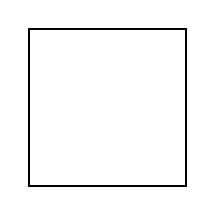
\begin{tikzpicture}[thick,scale=0.5]%
\draw (0,0) -- (4,0) -- (4,4) -- (0,4) -- cycle;
\end{tikzpicture}
Square
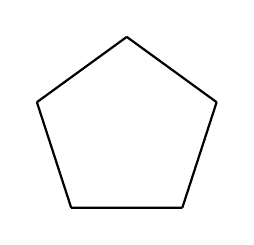
\begin{tikzpicture}[thick,scale=0.3]%
\draw \foreach \x in {18,90,...,306}{
		(\x:4) node{} -- (\x+72:4)
};
\end{tikzpicture}
Pentagon
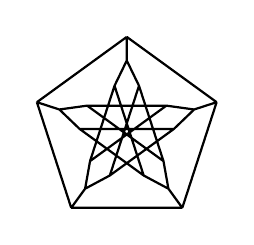
\begin{tikzpicture}[thick,scale=0.3]%
\draw \foreach \x in {18,90,...,306} {
	(\x:4) node{} -- (\x+72:4)
	(\x:4) -- (\x:3) node{}
	(\x:3) -- (\x+15:2) node{}
	(\x:3) -- (\x-15:2) node{}
	(\x+15:2) -- (\x+144-15:2)
	(\x-15:2) -- (\x+144+15:2)
};
\end{tikzpicture}
Some graph
\begin{tikzpicture}[thick,scale=0.4]%
\draw \foreach \x in {0,180} {	
		(\x:4) node{} - (\x+90:4)	
};
\end{tikzpicture}
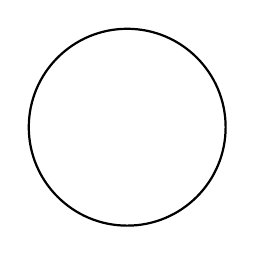
\begin{tikzpicture}
\draw[thick] (-1,0) circle (1.25);
\label{K$_{100}$}
\end{tikzpicture}

K 100
K5 
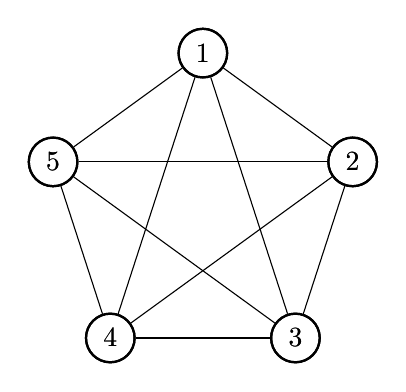
\begin{tikzpicture}[every node/.style={draw,circle,thick}]
\graph[clockwise, radius=2cm] {subgraph C_n [n=5,name=A] };
\graph[clockwise, radius=2cm] {subgraph I_n [n=5,name=B] };

\foreach \i [evaluate={\j=int(mod(\i+2+4,5)+1)}]% using Paul Gaborit's optimisation
in {1,2,3,4,5}{
	\draw (A \i) -- (B \i);
	\draw (B \j) -- (B \i);
}
\end{tikzpicture}
Peterson Graph
\begin{tikzpicture}
	content...
\end{tikzpicture}
 Cross-Cover graph

\subsection{Six Colour Theorem}
\textbf{Theorem: } A planar graph can be coloured with six colours.\\$\break$
1) Every planar graph has a vertex with atmost 5.\\
\textbf{Pf: } Let C be a component of a planar graph G. If V(C) $\leq$ 6, then every vertex of G has a degree of at most 5. If V(C) $\geq$ 6, then because it is a connected planar graph , we know that E(C) $\leq$ 3V(G) - 6. There fore the average degree is $\sum_{\emph{v$\epsilon$V(C)}}$$\frac{deg(v)}{V(C)}$ $\leq$ $\frac{6V(C)-12}{V(C)}$ = 6 - $\frac{12}{V(C)}$ $<$ 6. There is a vertex v of C whose degree is at most the average. Thus deg(v) $<$ 6 and so deg(v) $\leq$ 5.\\$\break$
2) To colour G, we proceed with induction on V(G)\\
\textbf{Pf: }If V(G) = 1, then G can be coloured with 1 (and therefore 6) colours.\\
For the induction step, choose a vertex V of G with degree at most 5. Colour G$\setminus$V with at most 6 colours (using inductive assumption). The neighbours are coloured by the colouring of G$\setminus$V \\ $\break$
\textbf{Proof: } Because deg(v) $\leq$ 5, at most five of the 6 colours are used as colours for the neighbours of v. Thusm there is one of the six colours not used to colour a neighbour of v, we can use this colour to colour v. Hence proved.\\ $\break$ 

\subsection{Five Colour Theorem}
\textbf{Theorem: } A planar graph can be coloured with five colours.\\$\break$
1) Every planar graph has a vertex with atmost 5.\\
\textbf{Pf: } Let C be a component of a planar graph G. If V(C) $\leq$ 6, then every vertex of G has a degree of at most 5. If V(C) $\geq$ 6, then because it is a connected planar graph , we know that E(C) $\leq$ 3V(G) - 6. There fore the average degree is $\sum_{\emph{v$\epsilon$V(C)}}$$\frac{deg(v)}{V(C)}$ $\leq$ $\frac{6V(C)-12}{V(C)}$ = 6 - $\frac{12}{V(C)}$ $<$ 6. There is a vertex v of C whose degree is at most the average. Thus deg(v) $<$ 6 and so deg(v) $\leq$ 5.\\$\break$
2) To colour G, we proceed with induction on V(G)\\
\textbf{Pf: }If V(G) = 1, then G can be coloured with 1 (and therefore 6) colours.\\
For the induction step, choose a vertex V of G with degree at most 5. Colour G$\setminus$V with at most 6 colours (using inductive assumption). The neighbours are coloured by the colouring of G$\setminus$V \\ $\break$
\textbf{Problem: } Deg(v) = 5. Because K$_5$ ia not planar, some two of the neighbours of v are not adjacent.\\
\textbf{Solution: }Let there be u and v. There two are not adjacent. Delete the edges from u to the other three neighbours of v \& contract to v the edge uv and v as to create a smaller graph G'.\\ $\break$
\textbf{Proof: }Continuing further from the solution, we see that by colouring G' with 5 colours by induction and colouring u and w, with the colour of the contracted vertex, every one else with their colour in G'. Since u, w have the same colour, neighbours of u and v have at most 4 colours in G$\setminus$v. This leaves the fifth colour for v.\\ $\break$
\subsection{K$_{3,3}$ is not planar}
\textbf{Lemma: }If a planar graph has no cycle and has atleast three vertices, then every face boundary has length $\geq$ 4.\\$\break$
\textbf{Corollary: }If G is a connected planar graph with $\geq$ 3 vertices and no 3 cycle, then E(G) $\leq$ 2V(G). \\ $\break$
So by using this above corollary K$_{3,3}$ is not planar
\section{Kuratowski's Theorem:}
A graph is not planar if and only if it contains a subdivision of either K$_5$ or K$_{3,3}$

Fig 1 and Fig 2 to be embedded here.

\chapter{Matchings}
\section{Matching or Matching in Graphs}
A \emph{matching} in a graph \emph{G} is a set M of edges of G, no two of which are incident with a common vertex. $\break$

Fig 3 and Fig 4\\ $\break$

For any matching M in a graph, 2$\mid$M$\mid$ $\leq$ $\mid$V(G)$\mid$. $\break$

A \emph{perfect Matching}  in a graph G is a matching \emph{M} in \emph{G} such that 2 = $\mid$V(G)$\mid$  \\ $\break$

The empty graph with at least one vertex has no perfect matching. Notice $\phi$ is a matching. \\ $\break$
\textbf{Note:} Even cycles have perfect matching. If $\mid$V(G)$\mid$ is odd then \emph{G} does not have a perfect matching \\ $\break$

In a K$_{p,q}$ graph we get the min\{p, q\} giving us the largest matching size.

\subsection{Covers or Covering the edges of a graph}
A cover of a graph G is a set \emph{C} of vertices such that every edge is incident with at least one vertex in C. \\   $\break$
\textbf{Fact: } If M is a matching and C is a cover in G, then $\mid$M$\mid$ $\leq$ $\mid$C$\mid$ .\\ $\break$
In a \emph{Cycle} of length \emph{n}: \\
the size of a largest matching is $\lfloor$ $\frac{n}{2}$ $\rfloor$\\
the size of a smallest cover is $\lceil$ $\frac{n}{2}$ $\rceil$ \\
In a K$_n$ graph:\\
the size of the matching $\lfloor$ $\frac{n}{2}$ $\rfloor$\\  
the cover for the cycle is: n-1\\ $\break$

In a K$_{p,q}$ complete graph (with p $\leq$ q):\\
the size of the matching is: p\\
the size of the cover is: p \\ $\break$				

\textbf{Lemma: } If \emph{M} is a matching and C is a cover then  $\mid$M$\mid$ $<$ $\mid$C$\mid$.\\ $\break$

\textbf{Proof: } Let e = uv be an edge in M. By definition, either u or v is in C (or both), without loss of generality, assume it is u. Let e' be a different edge in M. One of the endpoints of e'(w) is in C. Can u = w? By definition of the matching, e and e' share no endpoints, so u $\neq$ to w. There are $\mid$M$\mid$ edges un M. Each yields a unique  vertex in C $\rightarrow$ $\mid$M$\mid$ $\leq$ $\mid$C$\mid$\\ $\break$
Maximum mathcing a alaregest matching G. (No matching exist with more edges)\\
If the size os a maximum matching is $\frac{n}{2}$, then it is a  perfect\\ $\break$
Minimum cover is a smallest cover in C. \\ $\break$
\textbf{Lemma: }If M is a matching and C is a $\mid$ M $\mid$ = $\mid$C$\mid$ then, M is a maximum matching and C is the minimum cover.\\ $\break$
\textbf{Proof: }Let M* be a maximum mathcing, then $\mid$ M* $\mid$ $\leq$ $\mid$ C$\mid$ = $\mid$ M $\mid$. M has at least as many edges as M*(which is a maximum matching). So M is also a maximum matching. Let C* be a minimum cover. $\mid$ C* $\mid$ $\geq$ $\mid$ M$\mid$ = $\mid$ C $\mid$. So C is also a minimum cover. \\ $\break$
\textbf{Lemma: }If M has an augmenting path then i is not a maximum matching\\ $\break$
\textbf{Proof: }Let P be the augmenting path. The edges alternate between being in M and not being in M. The endpoints are unsaturated. More edges of P are not in M than are in M (one more). Replace the edges in M $\cap$ P with the edges in P set difference M. New matching M'. If v $\epsilon$ P is saturated by M. We removing the edge in M is incident to v and replacing it with one in M'. If v $\epsilon$ P is unsaturated, we only add one edge incident to v to form the matching M'.. M' is a matching $\mid$M'$\mid$ = $\mid$ M $\mid$ is not a maximum matching.\\ $\break$

\subsection{Augmented Paths}
An alternating Path is a path in  \emph{G} where the edges alternate between being in M and not being in M. An augmented Path is an alternating path where its endpoints are unsaturated.\\ Odd length\\ First + Last edge not in the matching

A vertex is a saturated by a matching M if it is incident to an edge in M. Otherwies it is unsaturated which is also called exposed. In a perfect matching, all vettices are saturated. If there's no perfect matching, at least one vertex is unsaturated in any matchings. $\break$

\textbf{Lemma: }Let \emph{G} be a graph with matching M. If there is a M - augmented path in \emph{G}, then M is not a maximum matching(swap the edges of the ones in M with the edges which are not in M)

\textbf{Lemma: }If M is not a max matching then it has an augmenting path. Will be done in tutorial
\\Let \emph{G} be a graph with bipartition A, B and let M be a matching of \emph{G}.\\
$\bullet$ Let X$_0$ be the set of vertices in A not saturated by M.\\
$\bullet$ Let Z be the set of vertices in \emph{G} joined to a vertex in X$_0$ by an alternating path.\\
$\bullet$ If there is an augmenting path use it to update the matching.\\
$\bullet$ Otherwise: X = A $\cap$ Z. \\ \hspace{56px} X = B $\cap$ Z \\ \hspace{56px} Cover: C = Y $\cup$ (A$\setminus$X)

Figure here

X$_0$ = \{b, e\}\\
Alternating Paths (Start from b$\setminus$e)
\{b,e,4,5,a,d,1,2,3\}

Figure 2 here

X$_0$ = \{e\}\\
Z = \{e, 4, 5, b, d\}\\

In order to have a augmenting path, Z must include an unsaturated vertex not in  X$_0$. Since Z does not contain 3 there is no augmenting path\\

X = A $\cap$ Z = \{b, d, e\}\\
Y = B $\cap$ Z = \{4, 5\}\\
C = Y $\cup$ (A $\setminus$ X) = \{4, 5\} $\cup$ \{a, c\} = \{4, 5, a, c\} is a min cover.\\ $\break$

\textbf{Lemma: }Let M be a matching of a bipartite graph with partition A, B. Then  \\
a) There is no edge from X to B$\setminus$Y.\\
b) C = Y $\cup$ (A$\setminus$X)  is a cover.\\
c) There is no edge of M from Y to (A$\setminus$X).\\
d) If u is the set of unsaturated vertices in Y then $\mid$M$\mid$= $\mid$C$\mid$ - $\mid$U$\mid$. \\
e)there is an augmenting path to each vertex in U.\\ $\break$

\textbf{Proof: } a) Suppose there is an edge where u $\in$ X, v $\in$ B $\setminus$Y. There is an alternating oath P from X$_0$ to u P' = P + uv. uv is not an edge of M. Alternating path to v. So V should be in Z.\\
b) Edges from:\\
X $\rightarrow$ Y - one end in Y and one end in C\\
X $\rightarrow$ B$\setminus$Y - don't exist by part a of the proof \\
A$\setminus$X $\rightarrow$ Y - both end in C\\
A$\setminus$X $\rightarrow$ B$\setminus$Y - one end in C\\
Hence C is cover\\ $\break$

c)Suppose the edge vw $\in$ M, v $\in$ A$\setminus$ X, w $\in$ Y, w $\in$ Z, so there is an alternating path from X$_0$ to w w$\in$B, so P has odd length (So to travel to the other set it should have an odd length length 1, 3, 5, ...). Starting from X$_0$, the first edge is not in M, so the last edge (incident edge to w) is also not in the matching. P' = P + vw is an alternating path and starts from X$_0$ to v.Thus v is in Z, hence it is in X. And since we said that v $\in$ A$\setminus$ X, it is a contradiction($\longrightarrow$!$\longleftarrow$)\\ $\break$
d) X $\rightarrow$ Y $\ast$ \\
X $\rightarrow$ B$\setminus$Y - does not $\exists$ \\
A$\setminus$X $\rightarrow$ Y - not in M by part c\\
A$\setminus$X $\rightarrow$ B $\setminus$Y $\ast$ - (2)\\
Number of edges X to Y in M.  $\mid$U$\mid$ unsaturated vertices in Y. $\mid$Y$\mid$ - $\mid$U$\mid$ saturated vertices in Y. One edge in M for each in M for each of these. Number of edges from X to Y in M = $\mid$Y$\mid$ - $\mid$U$\mid$.From (2) now, 0 unsaturated vertices in A$\setminus$X. $\mid$A$\setminus$X$\mid$ saturated vertices in A$\setminus$X. X$_0$ $\subseteq$ Z.So X$_0$ $\subseteq$ X. Number is equal to $\mid$A$\setminus$X$\mid$. So $\mid$M$\mid$ = $\mid$Y$\mid$ - $\mid$U$\mid$+$\mid$A$\setminus$X$\mid$. So by using part b of the proof, $\mid$M$\mid$ = $\mid$C$\mid$ - $\mid$U$\mid$. \\ $\break$
e) Let v $\in$ U. V is unsaturated and v $\in$ Y and since Y $\in$ B $\cap$ Z then v $\in$ Z. Then there is an alternating path from X$_0$ to v then it is an augmenting path.\\ Hence proved the lemma.


\section{Konig's Theorem}
\textbf{K$\ddot{o}$nig's Theorem: } In a bipartite graph, the maximum size of a mathcing is the minimum size of a cover.

\textbf{Proof: }Let M be a maximum matching. Then there is no augmenting path in G. Furthermore, $\mid$U$\mid$ = 0. So by part b from the previous lemma, C = Y $\cup$ (A$\setminus$X) and then it is a cover. By part d) we get that M = C.	$\square$.\\

-----

D is a set of vertices.

Neighbour set, denoted by N(D), is the set of vertices adjacent to a vertex in D
$\break$
\textbf{Halls' Theorem: } G is a bipartite graph with partition on A, B. G has a matching saturating every vertex in A if and only if every subset D of A satisfies\\ \hspace{200px} $\mid$N(D)$\mid$ $\geq$$\mid$D$\mid$

\textbf{Picture: } D = \{1, 2, 3\} \\
N(D) = \{a, c\}\\
$\vert$N(D)$\vert$ = 2 $<$ 3 = $\vert$D$\vert$
\section{Applications of Konig's Theorem}
\section{System of Distinct Represntatives}
\end{document}